%LaTeX template : http://systbio.org/files/SB_LaTeX_Template_txt_extension.txt
%Author instructions: http://www.oxfordjournals.org/our_journals/sysbio/for_authors/ms_preparation.html

\documentclass[12pt,letterpaper]{article}

%Packages
\usepackage{pdflscape}
\usepackage{fixltx2e}
\usepackage{textcomp}
\usepackage{fullpage}
\usepackage{natbib}
\usepackage{float}
\usepackage{latexsym}
\usepackage{url}
\usepackage{epsfig}
\usepackage{graphicx}
\usepackage{amssymb}
\usepackage{amsmath}
\usepackage{bm}
\usepackage{array}
\usepackage[version=3]{mhchem}
\usepackage{ifthen}
\usepackage{caption}
\usepackage{hyperref}
\usepackage{amsthm}
\usepackage{amstext}
\usepackage{enumerate}
\usepackage[osf]{mathpazo}
\usepackage{dcolumn}
\usepackage{lineno}
\pagenumbering{arabic}


%Pagination style and stuff
\linespread{2}
\raggedright
\setlength{\parindent}{0.5in}
\setcounter{secnumdepth}{0} 
\renewcommand{\section}[1]{%
\bigskip
\begin{center}
\begin{Large}
\normalfont\scshape #1
\medskip
\end{Large}
\end{center}}
\renewcommand{\subsection}[1]{%
\bigskip
\begin{center}
\begin{large}
\normalfont\itshape #1
\end{large}
\end{center}}
\renewcommand{\subsubsection}[1]{%
\vspace{2ex}
\noindent
\textit{#1.}---}
\renewcommand{\tableofcontents}{}
\bibpunct{(}{)}{;}{a}{}{,}

%---------------------------------------------
%
%       START
%
%---------------------------------------------

\begin{document}

%Running head
\begin{flushright}
Version dated: \today
\end{flushright}
\bigskip
\noindent RH: Tempo and mode in mammals evolution

\bigskip
\medskip
\begin{center}

\noindent{\Large \bf Tempo and mode in mammals morphological evolution around the K-Pg boundary}

\bigskip

\noindent {\normalsize \sc Thomas Guillerme$^1$$^,$$^2$$^*$, and Natalie Cooper$^1$$^,$$^2$}\\
\noindent {\small \it 
$^1$School of Natural Sciences, Trinity College Dublin, Dublin 2, Ireland.\\
$^2$Trinity Centre for Biodiversity Research, Trinity College Dublin, Dublin 2, Ireland.}\\
\end{center}
\medskip
\noindent{*\bf Corresponding author.} \textit{Zoology Building, Trinity College Dublin, Dublin 2, Ireland; E-mail: guillert@tcd.ie; Fax: +353 1 6778094; Tel: +353 1 896 2571.}\\
\vspace{1in}

%Line numbering
\modulolinenumbers[1]
\linenumbers

%---------------------------------------------
%
%       ABSTRACT
%
%---------------------------------------------

\newpage
\begin{abstract}

Massive global extinctions events are known to lead to major changes in ecosystems, especially with major shifts in species composition and species richness.

The Cretaceous-Paleogene boundary (K-T; 66Mya) represents a drastic global change in biodiversity. This event is linked to an extraterrestrial impact and a major volcanism event. Traditionally the K-Pg event was viewed as the extinction of dinosaurs and the rise of mammals. However, the last three decades of field palaeontology and macroevolutionary studies have weakened this simplistic view. Exceptionally diverse mammals appeared prior to the Paleogene and there is overwhelming evidence for a radiation of the avian-dinosaurs in the latest Cretaceous.

In this study, we use a character-space approach on multiple data sets of living and fossil mammals to investigate the variations in disparity and diversity in mammals since the Jurassic. We show that maximal disparity is achieved prior to the Paleogene and that there is no significant increase in diversity across the K-T boundary.

\end{abstract}

\noindent (Keywords: morphological characters, Bayesian, Maximum Likelihood, topology, fossil, living)\\

\vspace{1.5in}

\newpage 

%---------------------------------------------
%
%       INTRODUCTION
%
%---------------------------------------------

\section{Introduction}

%-Macroevolution / niches / crisis in biodiversity
%-Diversity in mammals is known to increase blablabla (Stadler)
%Cheeky selling line: in the context of the anthropocene extinction event, blabalbal
%-However, not much is known about the disparity. We think disparity is a more functional measure of biodiversity since it is expected that more disparate species occupies more disparate niches and therefore have a globally more important role in the ecosystems.
%-We use a novel approach for looking at disparity as the spread of the data in a N dimensional character-space (centroid - Finlay Cooper)
%-Problem with timing the events (O'Leary vs Meredith). Here we look at disparity on total evidence trees that contain morphological information but are backed-up by molecular data.


Abiotic and biotic changes can have a cascade effect on biodiversity and lead to drastic changes in species richness and composition. %Cheeky first line?
%Mass extinction leads to species turnovers.
Mass extinctions events leads to the extinction of entire clades (e.g. Ammonoidea at the end of the Cretaceous) but also leads to radiation of new clades (e.g. whatever formaminifera \cite{Erwin1998344} during the Cenozoic).
These biodiversity turn-over are consider to be due to niche replacement where the clades that suffers mass extinction (e.g. Brachipoda during the Permian-Triassic extinction event) leads vacant ecological niches that can be filled by a new unrelated clade that undergoes an adaptive radiation (e.g. Bivalvia after the Permian-Triassic extinction).  

However, this niches emptying/refilling concept is vague (cite cite cite) and the timing of the extinction event is crucial to determine if clades go exctinct and radiate due to niches emptying/filling.
%But it's complicated to determine if the clade after the extinction event undergoes an adaptive radiation because of the timing. Theoretically, the clade radiating in the empty niche should be significantly more specious after the extinction of the other clade.
It is therefore crucial to understand the real tempo and mode of a clade's evolution through time to be able to determine if it radiates because of niche availability let vacant by previous extinctions. Therefore, in a context of current global biotic and abiotic changes, resolving this question is crucial to understand the effect of mass extinction events on biodiversity.

The most recent mass extinction event, the Creatceous-Paleogene (K-Pg) extinction is really well studied geological with accurate dating of the events (cite) as well as the various causes and effects (cite).
%The Cretaceous-Paleogene (K-Pg) extinction is really well studied (cite cite cite) with good information on the timing of the event (66 Mya (cite)) and the causes of the extinction. But more is known about invertebrates than about vertebrates %The effect on invertebrates is also well understood.
However, there is still debate on the effect of the extinction on certain vertebrate groups (e.g. birds, crocodiles, mammals).

Within mammals, it still debated whether the eutherian group (crown and stem placentals) radiated after the K-Pg extinction because of the niche vacancy due to the extinction of non-avian dinosaurs (cite cite cite) or if eutherian mammals diversified during the Cretaceous and where not significantly affected by the K-Pg extinction (cite cite cite).
%Differences in interpretation of mammal tempo and mode is probably due to the data and the methods
The different views on the tempo and mode of diversification of placental mammals (post or pre K-Pg) is probably due to the differences in data and in methods. Studies advocating a pre K-Pg radiation are usually based on neontological data and probabilistic phylogenetic methods (Meredith and others) as post K-Pg radiation studies are based on palaeontological data and cladistic methods (O'Leary and others). Also it is important to note that, in the context of a niche filling (i.e. adaptive) radiation, diversity and speciation are only indirect proxys for looking at niche occupancy (i.e. the more speciation events, the more a clade should be succesfull in a niche).

One solution to resolving this apparent conflict is to use all the data available with the state-of-the art methods in phylogenetics along with better methods to measure the niche occupancy.
%Solution = use TEM (tip dated) and disparity
Another way to look at the tempo and mode in mammals evolution is to use all the data available to look at the diversification pattern (Total Evidence and tip dating) and to look at the diversity in morphologies (i.e. disparity) as a better proxy for niche occupancy (i.e. the more diverse morphologies, the more diverse niches are expected to be occupied).

In this study, we apply a new disparity through time (DTT) approach based on morphological data and phylogenetic time slicing. We apply this methods to data sets containing morphological data for both living and fossil taxa as well as molecular data for living taxa (TEM) and phylogenetic trees using Total Evidence data and dated using the tip-dating method. 
%In this study, we use integrative phylogenetic data (Total Evidence and tip dating) and a disparity through time approach to look at the changes in disparity in mammals around the K-Pg boundary. + null models of evolution (brownian)
We test if the K-Pg event let to a adaptive radiation of eutherian mammals into the vacant morphological niches that followed the extinction event. We expect to see a significant increase in disparity during the Cenozoic if the eutherian mammals did actually underwent an adaptive radiation.

We found that there is no increase in cladistic disparity after the K-Pg event and that actually the disparity in mammals picked during the K-Pg event.
%---------------------------------------------
%
%       METHODS
%
%---------------------------------------------

\section{Methods}

%To put somewhere:
%Methodological improvements
%Distance matrix: we use Graeme's MORD that more accurately reflects distances between taxa
%Disparity: we use the centroid distance \cite{finlay2015morphological} that is a clear and easily-interpretable method that is less dependent from diversity (see supplementaries)
%Time: we use Total Evidence Tip dated trees that are more accurate because they use probabilistic methods to estimate morphological phylogenetic distance (Wright) and provide more accurate ages of diversification events (Ronquist).
%Disparity through time: Finally, we use a novel method (to our knowledge) to look at the diversity through time. Instead of calculating the disparity of all species present in a time interval (e.g. Butler and Brusatte), we calculate disparity at a set of arbitrary and equidistant points in time. This new method provides a finer grain resolution of the evolution of diversity through time as well as two well defined models of character evolution (equilibrium - random, acctran, deltran - and continuous - proximity) contrary to the time interval method that assumes only punctuated equilibrium as a evolutionary model for morphological characters.



\subsection{Data}
For exploring the tempo and mode in mammalian evolution, we used the morphological matrices and total evidence tip dated trees \cite{ronquista2012} from \cite{MEE3:MEE312084} (103 taxa and 446 morphological characters) and \cite{beckancient2014} (102 taxa and 421 morphological characters). Both studies respectively ranges from the 310 Million years ago (Mya - Late Carboniferous) and 170 Mya (Middle Jurassic) to the present and focusing Mammaliamorpha up to the family level \cite{MEE3:MEE312084} and focusing on Eutheria up to a genus level \cite{beckancient2014}. We chose these two data sets because they both have similar cladistic properties (i.e. similar number of taxa and morphological characters) and both use the same phylogenetic method (total evidence tip dated trees \cite{ronquista2012}). However, both matrix differs on their taxonomic focus (Mammaliamorpha \textit{vs.} Eutheria) and their temporal range (310 to 0 Mya \textit{vs.} 170 to 0 Mya). To include the @span@ of each taxa in our analysis, we collected all the first and last occurrences datum for each taxa that occurred for more than our minimal time resolution (one million year, see below). This data were collected from the Paleobiology Database on @date@. Additionally, because both datasets don't sample the full diversity through time (and, to our knowledge, none does), we used the supertree from \cite{fritzdiversity2013} that is the most complete species level phylogeny of living mammals (93\% of the 5416 living mammals \cite{wilson2005mammal}) to calculate the changes in diversity through time in living mammals (see below).

\subsection{Ancestral states estimation}
For both matrices \cite{MEE3:MEE312084,beckancient2014}, we estimated the ancestral state of each character at every node in the tree. We used two slightly different Maximum Likelihood approaches to estimate the ancestral states. We preferred Maximum Likelihood methods on Bayesian methods because both methods have been shown to yield to similar results \cite{royer-carenzichoosing2013} but Maximum Likelihood methods are several orders of magnitude faster than Bayesian ones. We used the \texttt{rerootingMethod} function from the R package phytools 0.4-45 \cite{phytools}. This method performs a maximum likelihood estimation of the ancestral values and the variance of a Brownian motion process based on the re-rooting method of \cite{Yang01121995}. We followed \cite{Claddis} method for treating missing data at the tips as any possible observed state (e.g. if a character has two observed tips states 0 and 1 and a third tip has missing data (NA), the third tip will be considered as multi-state (0\&1) and the ancestor of these three tips can be estimated between the two following states: 0 and 1).

\subsection{Character-space estimation}
To explore the variation in mammals shapes through time, we use a cladistic-space approach \cite{Foote01071994,Foote29111996,Wesley-Hunt2005,Brusatte12092008,friedmanexplosive2010,toljagictriassic-jurassic2013}. Similarly to a morphospace analysis based on continuous morphological data(e.g. \cite{finlay2015morphological}), the cladistic-space is based on cladistic (or phenetic) data. Therefore, the cladistic-space is likely to be more influenced by the phylogeny than the morphospace \citep{Foote29111996,Wagner01011997}. However, discrete cladistic characters are still the best source for quantifying overall morphology for large and diverse groups \citep{Brusatte12092008}. Also, because of it's inherent combinatory properties, a cladistic-space is a finite theoretical space limited by the product of the number of character states. In fact, a cladistic-space will be overloaded if the number of taxa is higher than the product of the number of character states. Therefore it is straightforward to make sure that the character space does not contain more taxa than it's maximal capacity.

\subsubsection{Distance matrix and ordination}
The first step for creating the cladistic-space is to calculate the pairwise distance matrix between all taxa. We used the raw distances rescaled using Gower \cite{Gower71} dissimilarity rescaled using the arcsine of the square root (following Lloyd in prep). We also calculated the Generalised Euclidean Distance (GED) \cite{Wills2001} and the MORD distance (where the raw distances have been rescaled against the maximum possible observable distance  - Lloyd in prep) the results using both distances are available in the supplementary materials). We then ordinated the distance matrix using principal components ordination (PCO) to summarize the matrix and create the n dimensions of our cladistic-space. We used a PCO approach to be able to handle missing data and inapplicable characters \cite{lofgren2003,Wesley-Hunt2005}.

\subsection{Temporal division}
\subsubsection{Time slices}
We propose a new approach to look at the disparity through time by looking at the character-space at any time point in the phylogeny rather than considering the character-space in time intervals (e.g. \cite{Brusatte12092008,brusattedinosaur2012,toljagictriassic-jurassic2013}). In fact, the time intervals approach can suffer from several biases namely: (1) the time intervals duration is set arbitrarily and can distort the diversity or disparity in that time interval (for example, if stratigraphical ages are used, it is likely to increase the differences between two stratigraphical intervals since they where traditionally based on fossils morphological differences); (2) the time intervals method assumes that all characters evolve following a punctuate equilibrium rule (i.e. if a character between two time intervals, the character state is assumed to be constant during the whole time of the interval and then evolve quickly to reach the state in the second time interval and become constant again).

To address these issues, we propose a time slicing method that consists of only considering the ordinated distances of each taxa present only at a specific point in time. This methods allows to sample evenly which taxa are present through time in the phylogeny without arbitrarily group certain taxa together. For example, the slice at 0 Mya will contain only the extant taxa. When a particular particular point in time a branch instead of an edge, we propose two different models to determine whether to consider the ordinated distance from the ancestor edge or the descendant one.
\begin{enumerate}
\item{Punctuated model:} this model selects either the ordinated distance from the ancestor or the descendant edge. This model reflects punctuated equilibrium where the changes occur either at the start or at the end of a branch. In practice, we randomly chose the ordinated distance from the ancestor or the descendant edge each time. However, we also tested the model with the assumption that changes occurs early on the branch (ACCTRAN) or are delayed towards the next edge (DELTRAN). The result of both assumption are available in the supplementary.
\item{Constant model:} this models selects either the ordinated distance from the ancestor or the descendant edge according to the branch length separating the sampling point and the ancestor's edge. If the sampling point along the branch is lower than half the branch length, then the ordinated distance from the ancestor edge is selected. Else we selected the ordinated distance from the descendant edge. This model reflects constant evolution where changes rate are constant and cumulative along the branch (i.e. the hypothetical character state at any point in time will be the same to the closest observed state in time (ancestor or descendant edge)).
\end{enumerate}

\begin{figure}[!htbp]
\centering
    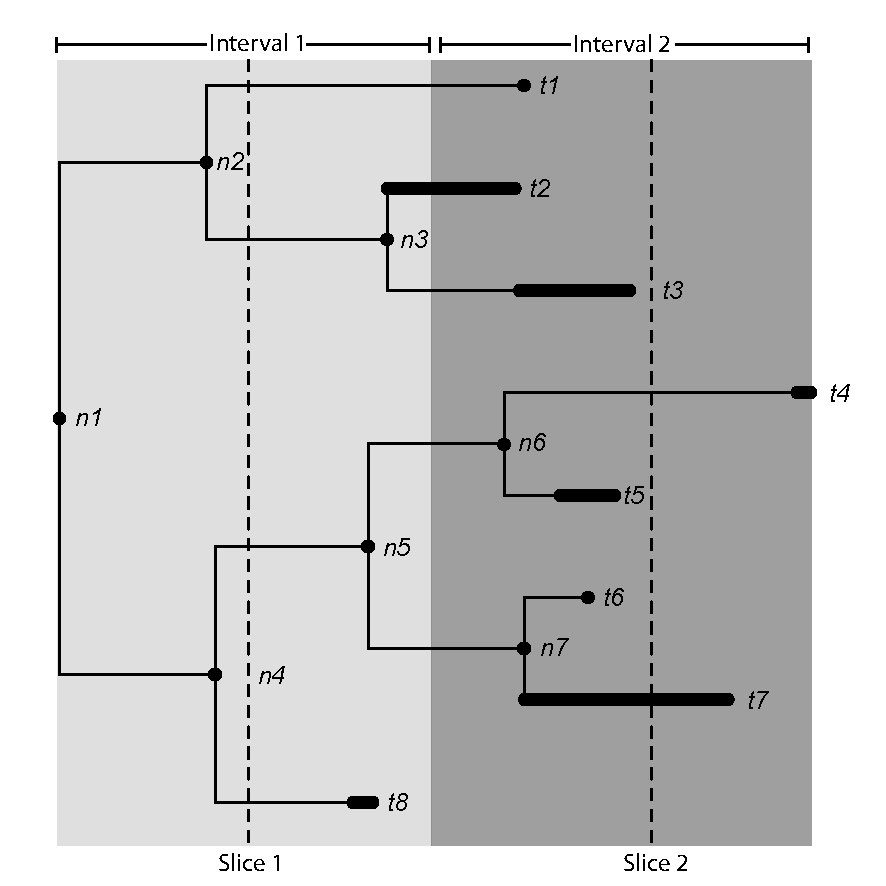
\includegraphics[keepaspectratio=true]{Figures/Slicing.pdf}
\caption{Differences in slicing method and intervals. Solid lines represent the First and Last Appearance Datum span. Interval 1 contains the following elements within the global character-space: taxa t2 and t8 and nodes n1, n2, n3, n4 and n5. Interval 2 contains the following elements within the global character-space: taxa t1, t2, t3, t4, t5, t6 and t7 and nodes n6 and n7. Slice 1 contains the following elements within the global character-space under the proximity model (constant evolution assumption): nodes n2 and n4. Slice 2 contains the following elements within the global character-space under the proximity model (constant evolution assumption): taxa t4 and t7.}
\label{slicing}
\end{figure}

This slicing method allows us for correcting for the two biases underlined above: (1) the time units are predefined (time steps) and not arbitrary anymore; (2) it is now possible to make two different assumption on how the different characters evolved through time (punctuate - randomly, ACCTRAN or DELTRAN - or constant). However, we also performed a time intervals approach available in the supplementary materials to compare our results to the previous method.


\subsection{Tempo and mode}
\subsubsection{Diversity}
Defined here as the number of taxonomic elements (OTUs) available in each matrix through time. We use as a base line, the diversity per million year 
\subsubsection{Disparity}
Defined here as the mean euclidean distance between each species and the centroid of the n dimension character-space.
%Disparity metrics should be calculated using a small number of PCO axes (12 \citep{Brusatte12092008}) encompassing a majority of the cumulative variance (63\% \citep{Brusatte12092008})
%Four disparity metrics can be calculated, the sum and product of the ranges and variance on the selected axes \citep{Wills1994}.
\subsubsection{Rarefaction}
To avoid bias due to diversity (disparity is expected to be smaller by chance when diversity decrease) we resample each time bin/slice to be equal to the minimal number of taxa available for all the bins/slices.
\subsubsection{Difference to null}
To test the statistical validity of the pattern in our data, we compared it to a null model where the character-space is generated randomly or under a constant birth death model. We compared the observed data to our null model for each time slice using the Bhattacharrya  coefficient (explain). We considered the observed disparity to be significantly different to the null models when less that 5\% of the distributions overlap (BC=0.05). Inversely, we considered them to be the same when 95\% of the data overlap (BC=0.95).

%---------------------------------------------
%
%       RESULTS
%
%---------------------------------------------

\section{Results}

%---------------------------------------------
%
%       DISCUSSION
%
%---------------------------------------------

\section{Discussion}
%Biases:
%-internal versus terminal branches
%-ancestral states reconstruction (solved by being conservative?)
%-poor sampling of living taxa (Guillerme & Cooper)
%---------------------------------------------
%
%       CONCLUSION
%
%---------------------------------------------

\section{Conclusion}


%---------------------------------------------

\section{Data availability and reproducibility}

\section{Acknowledgments}
Graeme Lloyd. 
%Simulations used the Lonsdale cluster maintained by the Trinity Centre for High Performance Computing and funded through grants from Science Foundation Ireland. %TG: I think they won't in the end

\section{Funding}
This work was funded by a European Commission CORDIS Seventh Framework Programme (FP7) Marie Curie CIG grant (proposal number: 321696).

\bibliographystyle{sysbio}
\bibliography{References}

\section{supplementaries}

\subsection{Ancestral states estimation}
We used both the \texttt{ace} function from the R package ape v. 3.2 \cite{paradisape:2004} and the 
\texttt{rerootingMethod} function from the R package phytools 0.4-45 \cite{phytools}. Both method perform a maximum likelihood estimation of the ancestral values and the variance of a Brownian motion process based on the re-rooting method of \cite{Yang01121995}. The two methods differ slightly in the calculation of the normalized conditional likelihoods but mainly on the way to treat missing data. We optimised the \texttt{ace} function for fast estimation by treating missing data in the matrix as an extra character (e.g. if a character has two observed tips states 0 and 1 and a third tip has missing data (NA), the ancestor of these three tips can be estimated between the three following states: 0, 1 and NA). For the \texttt{rerootingMethod}, we followed \cite{Claddis} method and treated the missing in the tips as any possible observed state (e.g. if a character has two observed tips states 0 and 1 and a third tip has missing data (NA), the third tip will be considered as multi-state (0\&1) and the ancestor of these three tips can be estimated between the two following states: 0 and 1). Both methods perform similarly but the implementation of the \texttt{ace} function has a slightly lower accuracy  but is three times faster than the one for the \texttt{rerootingMethod} function (see supplementaries).

\subsubsection{Time intervals}
We then divide our observed cladistic-spaces into sub cladistic-spaces representing the different stages of the character-space filling. For example, if at various points in time.
%The intervals should be a compromise between the resolution and the sample size and must be "sufficiently coards that nearly all generic first and last occurenaces can be unambiguously assigned" \citep{Foote01071994}.
Time intervals from 100Mya (Earliest Cenomanian, Late Cretaceous) to the present.
We count all the nodes/tips present in a given time interval.
Classic but artificially grouping data. The minimal bin size should contain at least two nodes/tips and sometime that involves having time intervals spanning accross tens of millions of years. Such long duration time intervals have no real biological meaning since it is unlikely that all of the nodes/tips present in the time interval did ever coexisted and had ever biological interactions together.


\subsection{Disparity}

\end{document}